\chapter{Realisieren}\label{ch:realisieren}
Dieses Kapitel zeigt die in der IPERKA-Phase «Realisieren» durchgeführten Arbeiten auf. In dieser Phase wird beschrieben wie der Lernende die Aufgabe umgesetzt hat und spricht Probleme bei der Umsetzung an.

\section{Endpoints für die Mindestanforderungen erstellen}
Die Reihenfolge, welche für diesen Abschnitt folgt, ist die Reihenfolge in der Implementiert wurde.

\subsection{MqInDTO}
Die Implementierung wurde mit der Erstellung von der MqInDto.java Klasse gestartet. Diese Klasse wird öfter in anderen Klassen verwendet und ist aus diesem Grund ein guter Startpunkt. Sie wurde mithilfe der MqOutDto.java Klasse als Beispiel erstellt, um die Konsistenz zwischen den verschiedenen DTO-Klassen beizubehalten. Sie beinhaltet mehrere Annotationen, um den Code kurz zu halten und Zeit bei der Implementation zu sparen:
\paragraph{@Data} \footnote{\url{https://projectlombok.org/features/Data}} generiert Getter, Setter und mehr .
\paragraph{@SuperBuilder} \footnote{\url{https://projectlombok.org/features/experimental/SuperBuilder}} erstellt ein Builder, welcher auch Felder von einer Superklasse verwenden kann.
\paragraph{@NoArgsConstructor} \footnote{\url{https://projectlombok.org/features/constructor}} generiert einen Konstruktor ohne Parameter.
\paragraph{@Schema} \footnote{\url{https://www.baeldung.com/swagger-parameter-vs-schema}} für die Kontrolle von spezifischen Definitionen wie Beschreibung oder Beispiele.
\paragraph{@NotNull} \footnote{\url{https://www.baeldung.com/java-notnull-method-parameter}} stellt sich, dass das Feld nicht «null» ist.\newline

\noindent Anschliessend wurden die Felder erstellt, mit den oben entsprechenden genannten Annotationen, die für die Tabelle im Frontend genutzt werden.

\subsection{MqInMapper}
Die Klasse MqInMapper.java hat die Annotation @Component, sodass Springboot diese Klasse instanziieren und sie mit allen angegebenen Abhängigkeiten injizieren kann.

Zwei Funktionen namens toMqInDto() und listToMqInDto() wurden in dieser Klasse erstellt. Die erste Funktion macht ein Mapping von MqTablePC (die ursprüngliche MqInPC-Klasse) zu MqInDto. Sie verwendet den Builder von der zuvor genutzten Annotation @SuperBuilder. Die zweite Funktion ruft die erste mithilfe von einem Stream auf. Der Stream wird verwendet, um jedes Element der Liste mit der Funktion toMqInDto aufzurufen. Dies wird mit .map() gemacht. Der Stream ermöglicht es, diese Aufgabe in einer kurzen Zeile zu schreiben, anstatt mit einem Loop jedes einzele Element der Liste hervorzuholen, zu mappen und anschliessend in einer zweiten Liste zu speichen. Die Funktion hat durch das nur insgesammt 3 Zeilen und vereinfacht das lesen.

\begin{verbatim}
	public List<MqInDto> listToMqInDto(List<MqTablePC> listOfMqTablePCs) {
		return listOfMqTablePCs.stream().map(this::toMqInDto).toList();
	}
\end{verbatim}

\subsection{MqInService}
Um die Struktur von eine Service vorzugeben, wurde ein Interface mit dem Namen MqInService erstellt. Dieses Interface wird später für die Klasse MqInServiceImpl.java und MqInServiceMockImpl.java verwendet und beinhaltet im Moment zwei Funktionen für das hervorholen von allen MqTables in der Datenbank und das ausführen von einem neuen Verarbeitungsversuch.

\subsection{MqInServiceImpl}
MqInServiceImpl wird vom Interface MqInService implementiert. Sie wird mit der Annotation @Service für Springboot als Service deklariert. Die Klasse enthält die vom Interface vorgegebene Funktion getMqTables(). Sie ruft eine Funktion von der Klasse MqTableDao (die ursprüngliche MqInDao-Klasse) auf die alle MqTable Einträge mit dem Status «Error» von der Datenbank hervorholt und sie auf 25 Einträge limitiert. Ein ändlicher Vorgehen hat die Funktion executeNewProcessingAttempt() die den Status vom MqIn auf NEW setzt.  

In dieser Klasse wurde auch ein Konstruktor erstellt. Bei dieser Implementierung trat ein Problem auf welches die Applikation nicht starten lies. Bei dem Parameter MqTableDao erschien die Meldung «Could not autowire. No beans of 'MqTableDao' type found.». Das Problem war, dass für die Klasse MqTableDao noch kein Bean erstellt wurde, obwohl die Klasse schon vorher existierte. Das Bean wurde anschliessend in der Klasse WebBackendAdminSpringConfiguration.java erstellt.

\subsection{MqTableDao}
Diese Klasse existierte bereits und war ursprünglich als MqInDao geplant. Durch das mussten nur die Funktionen hinzugefügt werden. Da es ein Interface ist, wurden nur die Namen und die benötigten Parameter hinzugefügt. Es wurden noch keine Bodys implementiert. Ausserdem wurden bei beiden Funktionen ein Kommentar erstellt. Der Kommentar beinhaltet eine kurze Beschreibung der Funktion und was sie zurückgibt. Mithilfe dieses Kommentars kann man jetzt über die Funktion drüberfahren und die Beschreibung wird als kurze Erklärung angezeigt.

\subsection{MqTableHibernateDao}
In der Klasse MqTableHibernateDao wird das Interface MqTableDao implementiert und muss durch das auch die neu erstellte Funktion implementieren.

Die Funktion nutzt einen CriteriaBuilder, um eine SQL-Query zu erstellen. Mit dieser Klasse konnte die Query so generiert werden, dass sie nach Enträgen filtert, die einen MQ\_IN\_STATUS von ERROR, als die Nummer Drei, haben. Die Query wird mithilfe von der Klasse CriteriaQuery bearbeitet und mit der Klasse Root können die einzelnen Spalten hervorgeholt werden, um sie zu vergleichen.

Um die Einträge auf 25 zu limitieren, musste noch die Klasse TypedQuery verwendete werden, welche dies ermöglichte.

\begin{verbatim}
	@Override
	public List<MqTablePC> findAllWithStatusErrorLimitedTo25() {
		CriteriaBuilder cb = getSession().getCriteriaBuilder();
		CriteriaQuery<MqTablePC> query = cb.createQuery(MqTablePC.class);
		Root<MqTablePC> mqTable = query.from(MqTablePC.class);
		
		query.where(
			cb.equal(mqTable.get(FN_MQ_IN_STATUS), ERROR)
		).orderBy(cb.desc(mqTable.get(FN_MODIFIED_AT)));
		
		TypedQuery<MqTablePC> typedQuery = getSession().createQuery(query);
		typedQuery.setMaxResults(25);
		
		return typedQuery.getResultList();
	}
\end{verbatim}

\noindent Für die zweite Funktion wurde ein CriteriaUpdateBuilder verwendet. Die restliche Implementation blieb fast gleich. Die Limitierung wurde entfernt und ein set() hinzugefügt, um den MQ\_IN\_STATUS auf NEW zu setzten.

\subsection{MqInResource}
Die Klasse MqInresource beinhaltet den geplanten Endpoint welcher im Arbeitspaket \ref{tab:realisieren-4.1} beschrieben wurde. Die Klasse wurde mit @RestController annotiert, sodass Spring weiss das diese Klasse Endpoints enthält. Sie hat ausserdem noch @RequestMapping, um den Pfad zu definieren und @RequiredArgsConstructor, welcher en Konstruktor generiert mit allen finalen und nicht-null Feldern.

Der Endpoint selbst hat drei Annotationen:

\paragraph{@GetMapping} \footnote{\url{https://www.geeksforgeeks.org/spring-postmapping-and-getmapping-annotation/}} deklariert diesen Endpoint als ein GET-Request.
\paragraph{@Operation} \footnote{\url{https://www.baeldung.com/swagger-operation-vs-apiresponse}} beschreibt die Funktion von diesem Endpoint.
\paragraph{@RequirePermission} \footnote{Vom Projekt CardX implementiert} stellt die Befugnis von diesem Endpoint ein. \newline

\noindent Der Endpoint selbst greift nur auf die erstellte Funktion in der Klasse MqInService.java zu und Mapped das erhaltene Resultat mithilfe des Mappers bevor er es wieder zurück sendet.

Der zweite Endpoint für das aussführen von einem weiteren Verarbeitungsversuch ist gleich aufgebaut wie der erste mit zwei Unterschieden. Er hat zwei andere Annotationen. Einerseits wurde der @GetMapping mit einem @RequestMapping ersetzt, sodass Spring weiss, dass es die Requests zu den richtigen Endpoints verweisen kann. Ausserdem hat dieser Endpoint ein Parameter namens id. Dieser Parameter wird vom RequestBody befüllt und muss deshalb mit @RequestBody annotiert werden.

\section{Die Seite und Tabelle im Frontend erstellen}

\subsection{Erstellung der Tabelle}\label{ch:creation-of-table}
Für die Erstellung der Tabelle wurde eine mq-in.service.ts-Klasse erstellt. Diese wird für die Requests an das Backend verwendet und beinhaltet die Funktion getAllMqInsLimitedTo25(), um alle MqIns von der Datenbank zu laden, und executeNewProcessingAttempt(id: number), die für die erneute Ausführung von einem Verarbeitungsveruch zuständig ist. Beide Funktionen rufen ihren erstellten Endpoint auf, welcher für das Frontend vom Projekt generiert wurde.

Diese Generierung kann mithilfe der Annotationen bei den entsprechenden Endpoints die HTTP-Requests generieren. Durch die generierte Swagger Datei wird eine zweite JSON-Datei generiert, die alle genötigten Informationen beinhaltet und im Modul Interface als web-backend-admin-api-.json gespeichert wird. Ein Plugin im Frontend nutzt anschliessend diese Datei, um die HTTP-Requests zu generieren.

Die Generierung vereinfachte die Nutzung von HTTP-Requests und hat die entsprechende Implementierung beschleunigt. Die Tabelle für die MqIns wurde durch das schnell erstellt und die ersten Einträge waren sichtbar auf der Seite.

\begin{figure}[H]
	\begin{center}
		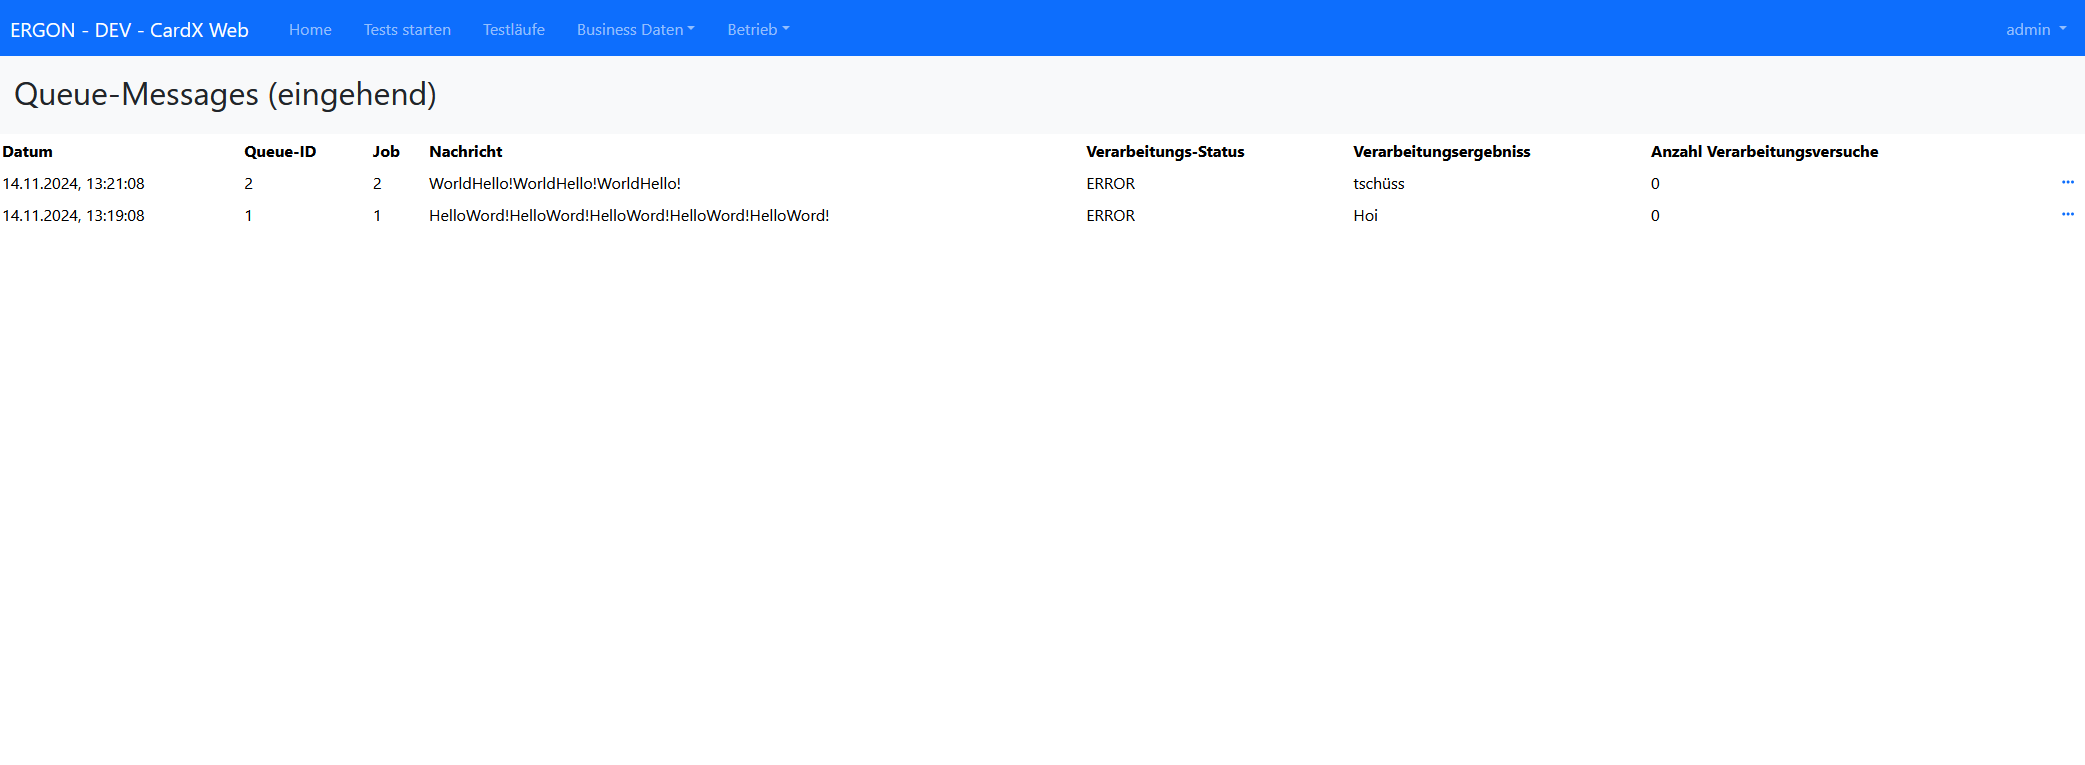
\includegraphics[width=1\textwidth]{ressourcen/4.2_Tabelle}
		\caption[Aktueller Stand der Tabelle]{Aktueller Stand der Tabelle}\label{fig:4.2-tabelle}
	\end{center}
\end{figure}

\subsection{Anzeigen der ganzen Nachricht}
Für das Anzeigen der ganzen Nachricht wurde eine neue Map erstellt, welche als Key die ID des MqIns und als Value einen Boolean enthält. Diese Map wird immer beim Aufruf der Seite gefüllt, nach dem die MqIns geladen wurden. Durch diese Map kann die ganze Nachricht angezeigt und anschliessend wieder verkürzt werden. Die eine Funktion setzt den entsprechenden Wert jedes Mal um, wenn man auf den Knopf «ganze Nachricht anzeigen» oder «Nachricht kürzen» drückt.

\noindent Die kurze Nachricht wird angezeigt:
\begin{figure}[H]
	\begin{center}
		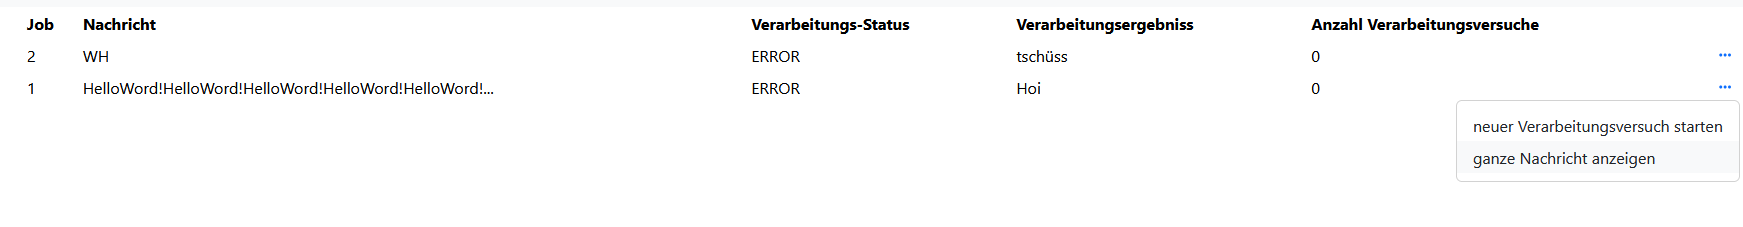
\includegraphics[width=1\textwidth]{ressourcen/Kurze-Nachricht}
		\caption[Gekürzte Nachricht]{Gekürzte Nachricht}\label{fig:show-shortend-version-of-message}
	\end{center}
\end{figure}

\noindent Die ganze Nachricht wird angezeigt:
\begin{figure}[H]
	\begin{center}
		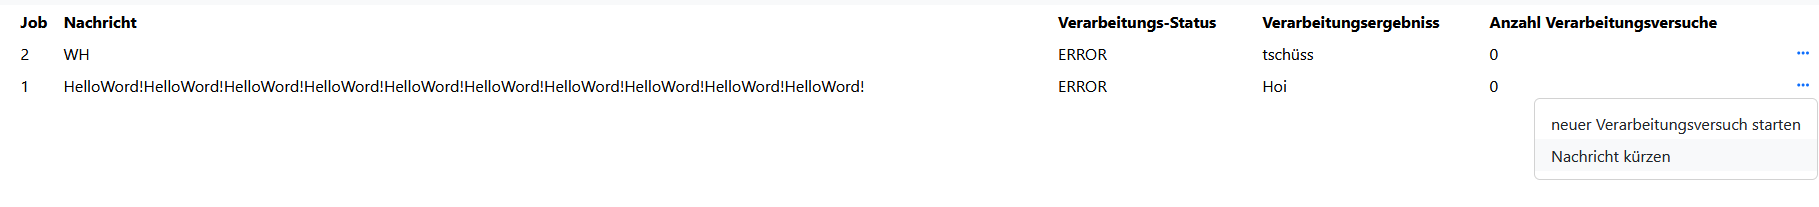
\includegraphics[width=1\textwidth]{ressourcen/Ganze-Nachricht}
		\caption[Ganze Nachricht]{Ganze Nachricht}\label{fig:show-hole-message}
	\end{center}
\end{figure}

\subsection{Erneutes Ausführen vom Verarbeitungsversuch}
Die Implementation für dieses Feature dauerte nicht lange, da, wie oben beschrieben \ref{ch:creation-of-table}, die HTTP-Requests generiert wurden und die Funktion nur noch verknüpft werden musste beim Drücken des Knopfs «neuer Verarbeitungsversuch starten». Dies war schnell gemacht und kostete nur im Backend ein wenig Zeit.

\begin{verbatim}
	private executeNewProcessingAttempt(id: number) {
		this.mqInService.executeNewProcessingAttempt(id)
		.subscribe({
			next: () => {
				this.loadMqIns();
			},
			error: (e: HttpErrorResponse) => {
				throw new ApiHttpErrorResponse('Die Verarbeitung der Queue konnte nicht neu gestartet werden.', e);
			},
		});
	}
\end{verbatim}

\noindent Diese Funktion ruft die Funktion executeNewProcessingAttempt() mit dem Parameter ID auf. Anschliessend führt die Subscribe folgende zwei Aktionen aus:

\paragraph{next:} wird ausgeführt, wenn der HTTP-Request erfolgreich war und die erwarteten Daten bereitgestellt wurden. In diesem Fall wird die Liste neu geladen.
\paragraph{error:} wird ausgeführt, wenn der HTTP-Request nicht erfolgreich war und ein Fehler während der Ausführung auftritt. Hier wird ein Fehler mit einer Nachricht geworfen.\newline

\noindent Danach ist die Backend-Anfrage fertig und war entweder erfolgreich oder nicht.


\newpage